%%%%%%%%%%%%%%%%%%%%%%%%%%%%%%%%%%%%%%%%%%%%%%%%%%%%%%%%%%%%%%%%%%%%%%%%%%%%%%%%
%2345678901234567890123456789012345678901234567890123456789012345678901234567890
%        1         2         3         4         5         6         7         8

\documentclass[letterpaper, 10 pt, conference]{ieeeconf}  % Comment this line out
                                                          % if you need a4paper
%\documentclass[a4paper, 10pt, conference]{ieeeconf}      % Use this line for a4 paper
\IEEEoverridecommandlockouts                              % This command is only needed 
%% % copyright info
%% \IEEEpubid{\makebox[\columnwidth]{978-1-5386-6133-8/18/\$31.00
%%         ~\copyright~2018 IEEE \hfill}\hspace{\columnsep}
%%         \makebox[\columnwidth]{ }}

% if you want to use the \thanks command
\overrideIEEEmargins
% See the \addtolength command later in the file to balance the column lengths on the last page of the document

% The following packages can be found on http:\\www.ctan.org
\usepackage{tikz}     % For adding axes to plots
\usepackage{graphicx} % For including PDFs
\usetikzlibrary{positioning}
\usepackage{balance} % For balancing the last column.

%% \usepackage{graphics} % for pdf, bitmapped graphics files
%\usepackage{epsfig} % for postscript graphics files
%\usepackage{mathptmx} % assumes new font selection scheme installed
%\usepackage{times} % assumes new font selection scheme installed
\usepackage{amsmath} % assumes amsmath package installed
\usepackage{amssymb}  % assumes amsmath package installed

%% Command for creating multiplie-line cells inside a table environment
\newcommand{\multilinecell}[2][c]{%
  \begin{tabular}[#1]{@{}c@{}}#2\end{tabular}}


\title{\LARGE \bf Effective Nonparametric Distribution Modeling \\ for Distribution Approximation Applications }

%% \author{Thomas C. H. Lux$^{1}$, Layne T. Watson$^{2,5}$, Tyler H. Chang$^{1}$, Li Xu$^{3}$, Yueyao Wang$^{3}$,\\ Jon Bernard$^{1}$, Yili Hong$^{4}$, Kirk W. Cameron$^{2}$% <-this % stops a space
%% \thanks{*This work was supported by the National Science Foundation Grant CNS-1565314.}%
%% \thanks{$^{1}$Doctoral candidate, Department of Computer Science, Virginia Polytechnic Institute and State University, Blacksburg, Virginia 24060, USA {\tt\small (tchlux at vt.edu)}}%
%% \thanks{$^{2}$Department of Computer Science, Virginia Polytechnic Institute and State University, Blacksburg, Virginia 24060, USA}%
%% \thanks{$^{3}$Doctoral candidate, Department of Statistics, Virginia Polytechnic Institute and State University, Blacksburg, Virginia 24060, USA}%
%% \thanks{$^{4}$Department of Statistics, Virginia Polytechnic Institute and State University, Blacksburg, Virginia 24060, USA}%
%% \thanks{$^{5}$Departments of Mathematics and Aerospace Engineering, Virginia Polytechnic Institute and State University, Virginia 24060, USA}%
%% }

\begin{document}

\maketitle
\thispagestyle{empty}
\pagestyle{empty}

%%%%%%%%%%%%%%%%%%%%%%%%%%%%%%%%%%%%%%%%%%%%%%%%%%%%%%%%%%%%%%%%%%%%%%%%%%%%%%%%
\begin{abstract}

Many fields of science rely on the collection of samples and estimation of true population distributions from those samples. There are several effective nonparametric methods for approximating a true distribution from empirical data, however it is unclear which methods produce the best approximations in practice. This work presents a case study on the effectiveness of various distribution approximations. Results show that piecewise linear approximations produce the smallest maximum absolute error, while the classic empirical distribution function (EDF) produces the smallest median absolute error as well as the smallest absolute error at lower percentiles when approximating a distribution from a sample. When building distribution prediction models, the piecewise quintic and cubic approximations produce the lowest absolute error at most error percentiles. These initial results encourage more research on the best methods of fitting empirical data with smooth functions to generate accurate distribution approximations.

\end{abstract}
%%%%%%%%%%%%%%%%%%%%%%%%%%%%%%%%%%%%%%%%%%%%%%%%%%%%%%%%%%%%%%%%%%%%%%%%%%%%%%%%

\section{INTRODUCTION}
\label{sec:introduction}

Empirical samples play a pivotal role in science. Experiments are run, data is recorded, and that data is used to draw conclusions about the \textit{truth}. When an experiment is run many times with varying outcomes, it is common to describe the truth as a random variable. In this work continuous (numeric) outcome random variables are considered. In this context, a random variable $X$ is precisely defined by its absolutely continuous \textit{cumulative distribution function} (CDF) $F_X$ and the derivative of the CDF, the \textit{probability density function} (PDF) $f_X$. As samples are drawn from $X$, the value of the CDF can be estimated at the sample points by measuring the probability at which other samples are less than or equal to that value. In this sense empirical data defines an empirical distribution function (EDF). The points that define the EDF are used to construct approximations of the true underlying CDF.

An approximation of a CDF can have varying levels of smoothness and, for empirical purposes the approximations are constructed over a closed interval. Piecewise polynomial functions (splines) provide the smooth approximations for animation in graphics \cite{herman2015techniques,quint2003scalable}, aesthetic structural support in architecture \cite{brennan2019measure}, efficient aerodynamic surfaces in automotive and aerospace engineering \cite{brennan2019measure}, and most importantly to this work they can provide accurate nonparametric approximations in statistics \cite{knott2012interpolating}. While polynomial interpolants or regressors apply broadly, splines are often a good choice because they can approximate globally complex functions while minimizing the local complexity of an approximation.

\begin{figure}
  \vspace{-.3cm}
  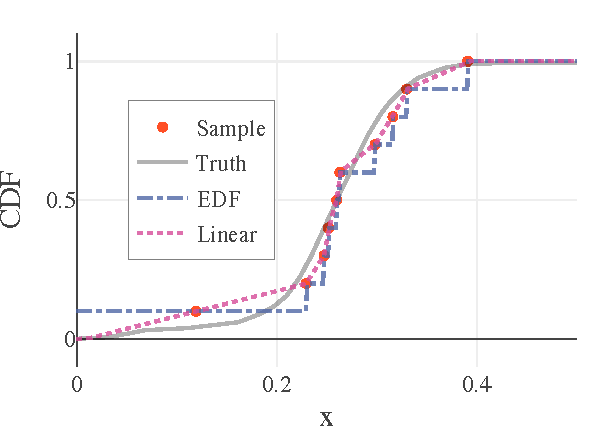
\includegraphics[width=.5\textwidth]{fl-sample-prediction.pdf}
  \caption{A demonstration of the linear fit and the classic EDF over a sample of 10 points. This data is normalized to be in the range $[0,1]$ and the right half of the domain is cropped out of this plot. Notice that the EDF points do not necessarily (and often do not) exactly equal the true CDF at any given position. The sampling inherently introduces variance into measurements of the CDF. This makes producing an accurate approximation difficult, as will be seen.
  \vspace{-.5cm}}
  \label{fig:sample-prediction}
\end{figure}

In this statistical work, the construction of a monotone interpolating spline that is continuous in its derivatives could be meaningfully useful \cite{ramsay1988monotone}. A function with $C^1$, and especially $C^2$ continuity could approximate a cumulative distribution function to a high level of accuracy with relatively few intervals. A twice continuously differentiable approximation to a cumulative distribution function (CDF) would also produce a corresponding probability density function (PDF) that is continuously differentiable, which is a desirable property many standard parametric distributions maintain.

There is publicly available software for monotone piecewise polynomial interpolation, including quadratic \cite{he1998monotone}, cubic \cite{fritsch1980monotone}, and (with limited application) quartic \cite{wang2004rational,piah2011improved,yao2018unconditionally} cases. Theory has been provided for the quintic case \cite{ulrich1994positivity,hess1994positive}. Recently an algorithm for the construction of monotone quintic splines has been produced as well (citation pending).%% \cite{lux2020algorithm}
This work considers the EDF, a linear interpolant, a monotone cubic spline interpolant, and a monotone quintic spline interpolant as candidate approximations.

In the next section, the methodology of this work is outlined and experimental setup is detailed. In Section \ref{sec:results}, three experiments related to the approximation of cumulative distribution functions are presented and analyzed. Finally Section \ref{sec:conclusion} concludes.


\begin{figure}
  \vspace{-.3cm}
  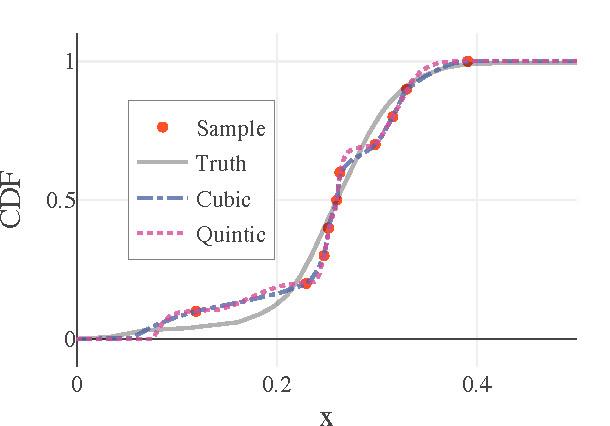
\includegraphics[width=.5\textwidth]{cq-sample-prediction.pdf}
  \caption{A demonstration of the monotone cubic and quintic spline interpolants over a sample of 10 points. This data is normalized to be in the range $[0,1]$ and the right half of the domain is cropped out of this plot. Notice that the difference between EDF points and the true CDF reduce the accuracy of first derivative (for both) and second derivative (for quintic) estimates in the interpolants, magnifying the error in the empirical estimations of CDF values.
  %% \vspace{-.5cm}
  }
  \label{fig:sample-prediction}
\end{figure}

%% ===================================================================
\section{METHODOLOGY AND DATA}
\label{sec:methodology}

In order to identify the best performing approximation techniques for distribution estimation, a case study on real-world data is presented and three experiments are run on that data to test various fits. First the accuracy of distribution approximations with varying sample sizes is studied, then the likelihood of any technique having the smallest maximum error is estimated, and finally the approximations are used to make predictions in a distribution prediction application similar to \cite{lux2018nonparametric}. Each experiment presents a unique, albeit with limited data, perspective on the quality of approximation provided by the four distribution approximation techniques.

The CDF modeling case study is constructed from a four-dimensional dataset produced by executing the IOzone benchmark \cite{iozone} on a homogeneous cluster of computers. Each node contains two Intel Xeon E5-2637 CPUs offering a total of 16 CPU cores with 16GB of DRAM. While the CPU frequency varies depending on the test configuration, the I/O from IOzone is performed by an ext4 filesystem sitting above an Intel SSDSC2BA20 SSD drive. At the time of data collection, Linux kernel Version 4.13.0 was used. The system performance data was collected over two months by executing IOzone  $10000$ times for each of a select set of $17$ system configurations, for a total of $170$ thousand executions of IOzone. A single IOzone execution reports the max I/O throughput in bytes per second seen for the selected test type. For this case study, only the results of a ``readers'' test are considered, where bytes are sequentially read from the SSD. The summary of the data for the experiments for this paper can be seen in Table \ref{tab:data_description}. Distributions of raw throughput values being modeled can be seen in Figure \ref{fig:throughput_histogram}.


The performance of approximation techniques that predict probability functions can be analyzed through a variety of summary statistics. The first two experiments study the distribution of absolute differences between approximated CDFs and the true CDFs. This distribution over many trials gives an idea of the \textit{expected} error. The last experiment in this work analyzes the max absolute difference between approximated and true CDFs, also known as the Kolmogorov-Smirnov (KS) statistic \cite{lilliefors1967kolmogorov} for its compatibility with the KS test.

The two-sample KS test is a useful nonparametric test for comparing two CDFs while only assuming stationarity, finite mean, and finite variance. The null hypothesis (that two CDFs come from the same underlying distribution) is rejected at level $p \in [0,1]$ when
 $$ KS > \sqrt{-\frac{1}{2}\ln\biggl(\frac{p}{2}\biggr)} \sqrt{\frac{1}{n_1} + \frac{1}{n_2}}, $$
with distribution sample sizes $n_1,n_2 \in \mathcal{N}$. For all applications of the KS test presented in this work $n_1 = n_2$.

Finally an example of the round-trip prediction methodology from known and predicted distributions to the calculation of error can be seen in Figure \ref{fig:prediction-example}. The Delaunay triangulation is a well-studied geometric technique for producing an interpolant \cite{lee1980two}. The Delaunay triangulation of a set of data points into simplices is such that there are no data points inside the sphere defined by the vertices of each simplex. For a $d$-simplex S with vertices $x^{(0)}$, $x^{(1)}$, $\ldots$, $x^{(d)}$, and functions $F_{x^{(i)}}$, $i=0$, $\ldots$, $d$, $y \in S$ is a unique convex combination of the vertices,
$$ y = \sum_{i=0}^{d} w_i x^{(i)}, \quad \sum_{i=0}^{d} w_i = 1, \quad w_i \geq 0, \quad i=0,\ldots,d, $$
and the Delaunay interpolant $F_y$ at $y$ is given by
$$ F_y = \sum_{i=0}^{d} w_i F_{x^{(i)}}. $$
In the case of these experiments, the file size, record size, thread count, and CPU frequency are first normalized to the unit hypercube. After normalization, Delaunay predictions are made via a leave-one-out method resulting in throughput data from five known configurations being used to predict one unknown throughput distribution. The Delaunay method is used to select the five source distributions as well as provide the convex weights associated with each of the source distributions that will most likely produce the predicted distribution.


\begin{figure}
  \vspace{-.3cm}
  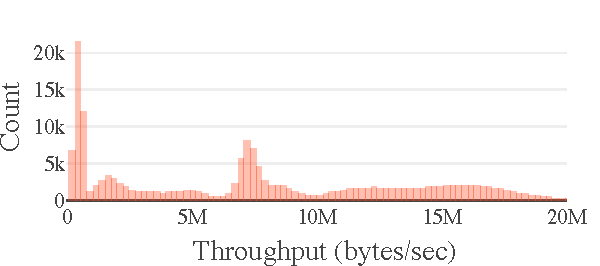
\includegraphics[width=.5\textwidth]{throughput-histogram.pdf}
  \caption{A histogram of all throughput values across the 17 unique system configurations and 170 thousand executions of a ``readers'' test in IOzone.}
  \label{fig:throughput_histogram}
\end{figure}

\begin{table}
  \centering
  \begin{tabular}{c|c}
    \hline
    \textbf{System Parameter} & \textbf{Values}\\
    \hline
    File Size (KB) & 4, 64, 256, 1024, 8192, 16384, 32768, 65536\\
    \hline
    Record Size (KB) & 4, 8, 16, 32, 64, 128, 4096, 8192, 16384\\
    \hline
    Thread Count & 8, 16, 24, 32, 40, 48, 56, 64\\
    \hline
    Frequency (GHz) & 1.2, 1.6, 2, 2.3, 2.8, 3.2, 3.5\\
    \hline
  \end{tabular}
  \caption{A description of system parameters considered for IOzone. Record size must be less than or equal to file size during execution. In all, $10$ thousand repeated trials are run at $17$ unique system configurations.
    \vspace{-.5cm}}
  \label{tab:data_description}
\end{table}


\begin{figure}
  \begin{tikzpicture}
    \node (img)  {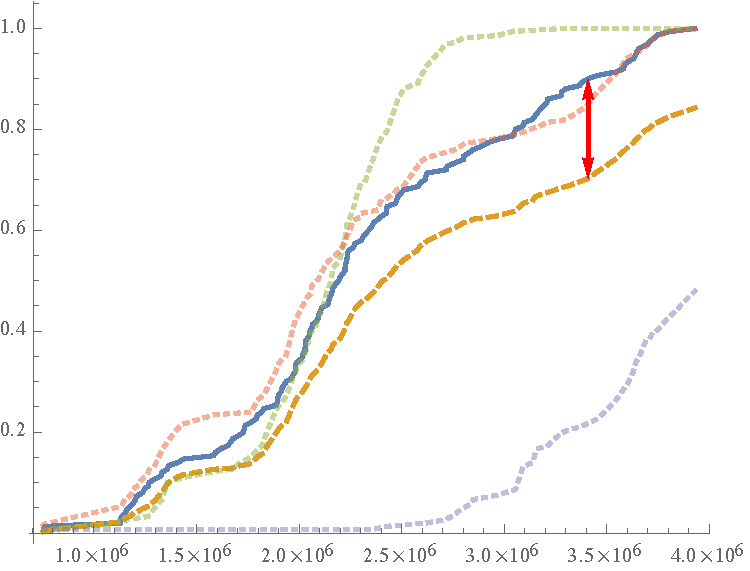
\includegraphics[width=0.4\textwidth,]{plot-delaunay-example-prediction.pdf}};
    \node[below=of img, node distance=1cm, yshift=1cm] {I/O Throughput};
    \node[left=of img, node distance=0cm, rotate=90, anchor=center,yshift=-0.7cm] {CDF Value};
  \end{tikzpicture}
  \vspace{-0.3cm}
  \caption{In this example, the general methodology for predicting a CDF and evaluating error can be seen. The Delaunay method chose three source distributions (dotted lines) and assigned weights \{.3, .4, .3\} (top to bottom at arrow). The weighted sum of the three known CDFs produces the predicted CDF (dashed line). The KS Statistic (arrow) computed between the true CDF (solid line) and predicted CDF (dashed line) is 0.2 for this example. The KS test null hypothesis is rejected by $p$-value 0.01, however it is not rejected by $p$-value 0.001.
  \vspace{-.1cm}}
  \label{fig:prediction-example}
\end{figure}


\section{RESULTS}
\label{sec:results}

All experiments that follow will consider the differences between CDF approximations given by the EDF, a linear interpolant, a monotone cubic interpolant, and a monotone quintic interpolant. In the first experiment, all four methods are used to approximate the ``true'' distributions of the ten thousand throughput values at each system configuration. One hundred random collections of $k$ samples are drawn from each true distribution for $k = 10$, $50$, $200$ and all methods are used to approximate the true distribution from each sample. In Figure \ref{fig:abs-error-dist}, the distributions of absolute difference between the ``true'' CDF and each approximated CDF at $1000$ equally spaced percentiles is shown. The sample of $50$ produces almost exactly half the errors observed with $10$ samples, and the error is roughly halved again when increasing to $200$ samples. Aside from the reduction in accuracy caused by sample size, most approximations appear to be nearly identical. When only $10$ samples are observed, the EDF has slightly less absolute error than other techniques between the median and third quartile. This difference is very minor, and difficult to observe.

\begin{figure}
  \vspace{-.3cm}
  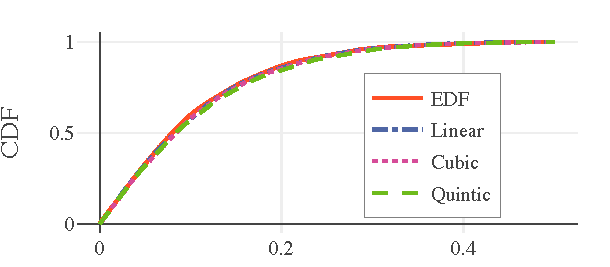
\includegraphics[width=.45\textwidth]{abs-errors-10-samples.pdf}
  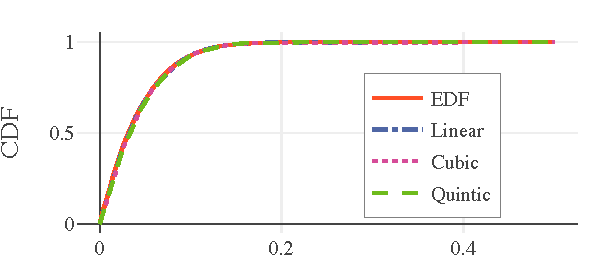
\includegraphics[width=.45\textwidth]{abs-errors-50-samples.pdf}
  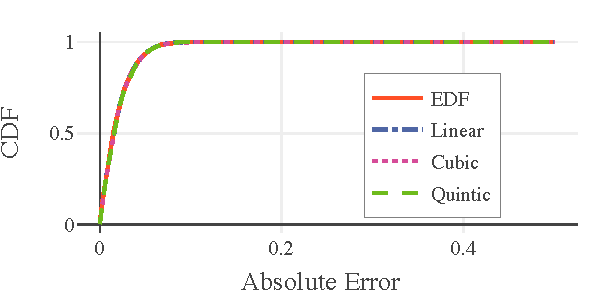
\includegraphics[width=.45\textwidth]{abs-errors-200-samples.pdf}
  \caption{The distribution of absolute errors with $10$ (top), $50$ (middle), and $200$ (bottom) samples for each approximation method. Notice that the EDF performs slightly better than other methods (more small absolute errors) when there are only $10$ samples. Given $50$ or more samples, all the approximations produced nearly identical errors.
  \vspace{-.5cm}}
  \label{fig:abs-error-dist}
\end{figure}

The second experiment considers the KS statistic (maximum absolute error) rather than the aggregate of errors. An increased collection of sample sizes is considered, with $k =$ 10, 20, 30, 40, 50, 60, 70, 80, 90, 100, 150, 200, 250, 300, 400, 500. For all $k$, 100 random samples of $k$ throughput values are drawn from the true distributions and approximate CDFs are constructed via each of the four methods. The error of each approximate CDF is measured at 1000 equally spaced percentiles and the maximum absolute error is recorded. At each sample size, Figure \ref{fig:ks-rank-0} depicts the probability that any given approximation method produces a distribution estimate with the lowest KS statistic. In this measure of error, the piecewise quintic and cubic approximations to the CDF provide the most accurate estimate of the true CDF. This result reveals that the chosen measure of error is important in determining which CDF approximation method is most suited to an applications. The EDF provides the lowest expected absolute error, however, the more smooth approximations appear to provide lower maximum absolute error.

\begin{figure*}
  \vspace{-.3cm}
  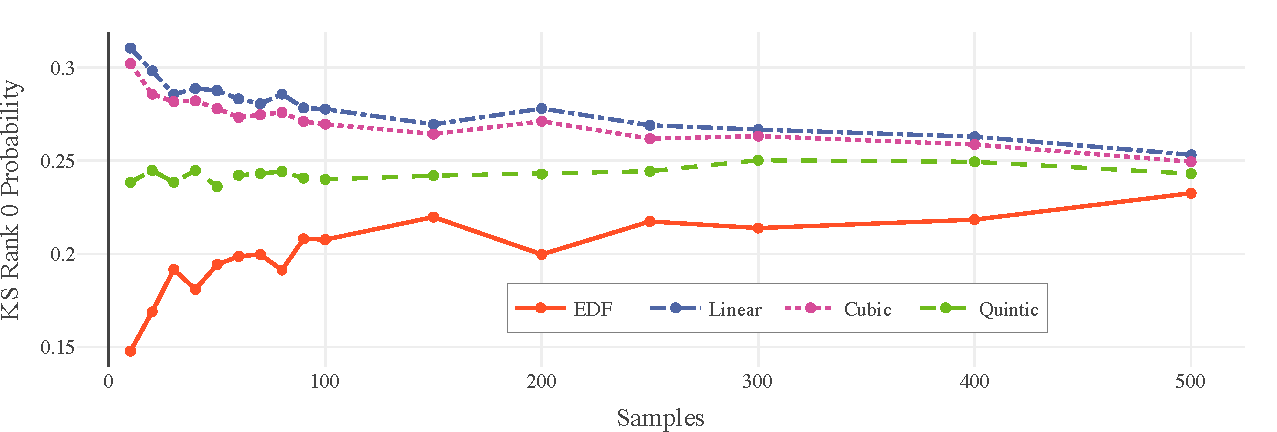
\includegraphics[width=1\textwidth]{KS-rank-0-probability.pdf}
  \caption{The probability that any one of the distribution approximation techniques has the lowest KS statistic among all the techniques when given a varying number of samples. Notice that the linear approximation remains the most likely to have the smallest KS statistic for all sample sizes, closely followed by the cubic.
  \vspace{-.5cm}}
  \label{fig:ks-rank-0}
\end{figure*}


The third experiment considers a distribution prediction application. In this case, the Delaunay method was applied to choose five source distributions and convex weights that will predict the throughput distribution at the system configuration with a 2.8GHz CPU frequency, 16 megabyte (MB) file size, 16MB record size, and 64 threads. This configuration is predicted because it is the only interpolation point (configuration inside or on the convex hull of other configurations) among the 17 available system configurations. An example of the prediction methodology can be seen in Figure \ref{fig:prediction-example}. The distribution of absolute errors measured at 1000 equally spaced percentiles of the true CDF for all four approximation methods can be seen in Figure \ref{fig:delaunay-errors}. In this case the piecewise quintic and cubic approximations provide the best predictions overall. The quintic and cubic methods produce smaller errors than the piecewise linear and EDF approximations at more than 90\% of measurements.

\begin{figure}
  \vspace{-.3cm}
  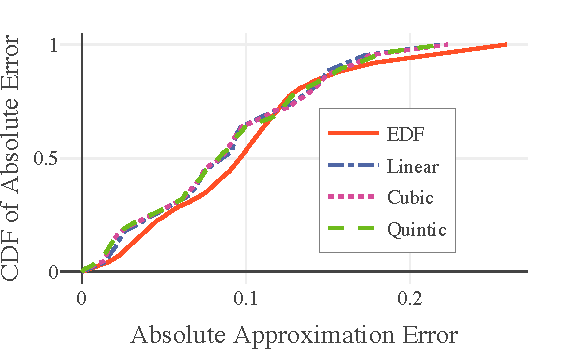
\includegraphics[width=.5\textwidth]{delaunay-predictions.pdf}
  %% 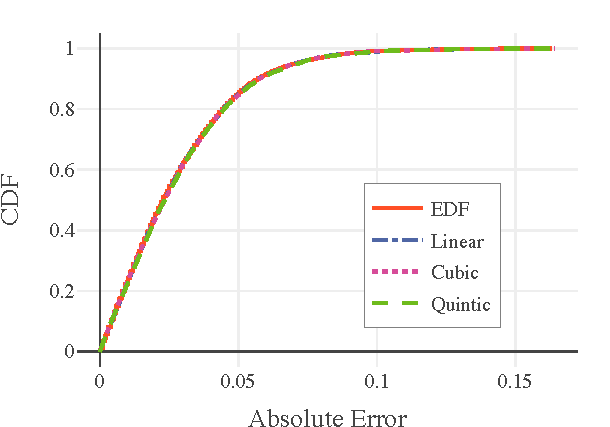
\includegraphics[width=.5\textwidth]{abs-errors-100-samples.pdf}
  \caption{The result of using Delaunay to predict distributions. Notice that the best performing, lowest error (to the left), approximation is the EDF. Interestingly, the piecewise linear fit does not produce results as accurate as the EDF. This likely has to do with the inherent smoothing that happens when multiple different EDFs are combined to make one prediction.
  \vspace{-.5cm}}
  \label{fig:delaunay-errors}
\end{figure}


The three experiments presented in this section have each tested a unique facet of distribution approximation. The first experiment analyzes the approximation of a distribution from a sample when measuring the aggregate absolute CDF approximation error; in this case the EDF largely produces the best approximations. The second experiment analyzes the maximum absolute error when approximating a CDF from a sample; in this case the monotone quintic and cubic spline interpolants are most likely to provide the best approximation. The third and final experiment analyzes the aggregate absolute error when predicting unobserved distributions, for which the monotone quintic and cubic splines produced the best overall CDF approximations.

%% \section{DISCUSSION}
%% \label{sec:discussion}

%% Discussion text..


\section{CONCLUSION}
\label{sec:conclusion}

This preliminary case study on the best functions for approximating cumulative distribution functions from empirical data has given some actionable insights. Specifically, the choice of error measure is important in deciding which distribution approximation method to apply to a sample. The standard empirical distribution function has the lowest expected absolute error when approximating a CDF given a sample of data. However, more smooth estimates like monotone quintic splines produce lower expected KS statistics (maximum absolute error), and are expected to have lower error in distribution prediction applications.

Future research may extend this case study to other data sets and include a more exhaustive distribution prediction test suite (experiment three). Tangentially, future work may target improved estimates of the first and second derivatives of the true CDF given a sample of data in order to reduce the approximation error of the monotone quintic and cubic spline methods.

\balance

\bibliographystyle{IEEEtran}
\bibliography{paper}


%% \newpage


%% \begin{figure}
%%   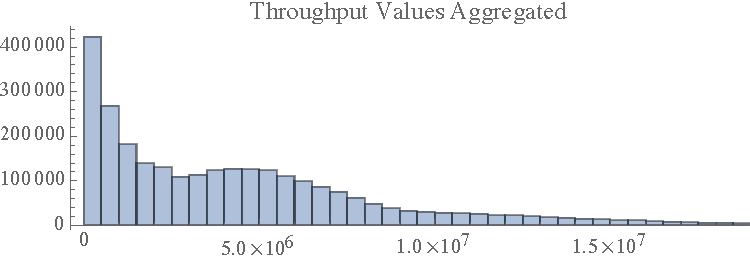
\includegraphics[width=.5\textwidth]{plot-histogram-throughput.pdf}
%%   \caption{Histogram of the raw throughput values recorded during all IOzone tests across all system configurations. The distribution is skewed right, with few tests having significantly higher throughput than most others.
%%   \vspace{-.5cm}}
%%   \label{fig:throughput_histogram}
%% \end{figure}

%% This paper presents a variability modeling case study with a five-dimensional dataset produced by executing the IOzone benchmark \cite{iozone} on a homogeneous cluster of computers. Each node contains two Intel Xeon E5-2637 CPUs offering a total of 16 CPU cores with 16GB of DRAM. While the CPU frequency varies depending on the test configuration, the I/O from IOzone is performed by an ext4 filesystem sitting above an Intel SSDSC2BA20 SSD drive. At the time of data collection, Linux kernel Version 4.13.0 was used. The system performance data was collected over two weeks by executing IOzone 150 times for each of a select set of approximately 18K system configurations, for a total of approximately 2.7M executions of IOzone. A single IOzone execution reports the max I/O throughput in kilobytes per second seen for the selected test type. The summary of the data components in $x^{(i)}$ for the experiments for this paper can be seen in Table \ref{tab:data_description}. Distributions of raw throughput values being modeled can be seen in Figure \ref{fig:throughput_histogram}.

%% Some mild preprocessing was necessary to prepare the data for modeling and analysis. All features were shifted by their minimum value and scaled by their range, mapping each feature independently into $[0,1]$. This normalization ensures each feature is treated equally by the interpolation techniques and should be performed on all data before building models and making predictions regardless of application. All 150 repeated trials for a system configuration were grouped with that configuration. The only nonordinal feature in this data is the test type. All test types were treated as different applications and were separated for modeling and analysis, i.e., predictions for the ``readers'' test type were made using only known configurations for the ``readers'' test type.

%% %% ===================================================================

%% \begin{figure}
%%   \begin{tikzpicture}
%%     \node (img)  {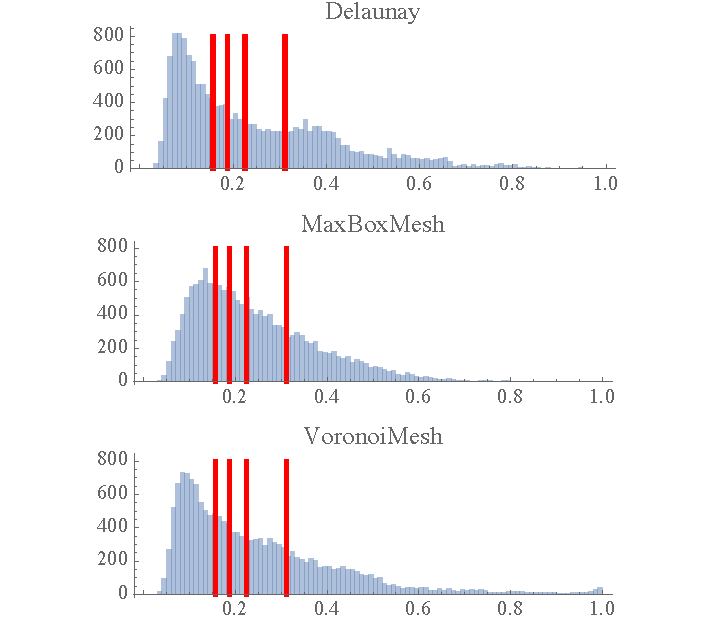
\includegraphics[width=0.5\textwidth,trim={1.5cm 0 0 0}]{plot-histogram-80_20-KS.pdf}};
%%     \node[below=of img, node distance=1cm, yshift=1cm] {KS Statistic for Predicted vs. Actual};
%%     \node[left=of img, node distance=0cm, rotate=90, anchor=center,yshift=-0.7cm] {Count of Predictions with Given KS Statistic};
%%   \end{tikzpicture}
%%   \caption{Histograms of the prediction error for each modeling algorithm from ten random splits when trained with 80\% of the data aggregated over all different test types. The distributions show the KS statistics for the predicted throughput distribution versus the actual throughput distribution. The four vertical red lines represent commonly used $p$-values \{0.05, 0.01, 0.001, 1.0e-6\} respectively. All predictions to the right of a red line represent CDF predictions that are significantly different (by respective $p$-value) from the actual distribution according to the KS test.
%%   \vspace{-.1cm}}
%%   \label{fig:ks_histogram_80_20}
%% \end{figure}

%% \begin{table}
%%   \centering
%%   \begin{tabular}{c|c|c}
%%     \hline
%%     \textbf{Algorithm} & \textbf{$P$-Value} & \textbf{\% N.H. Rejections} \\
%%     \hline
%%     \multilinecell{Delaunay\\Max Box Mesh\\Voronoi Mesh} & .05 & \multilinecell{58.4\\69.3\\61.9}\\
%%     \hline
%%     \multilinecell{Delaunay\\Max Box Mesh\\Voronoi Mesh} & .01 & \multilinecell{51.1\\58.4\\53.4}\\
%%     \hline
%%     \multilinecell{Delaunay\\Max Box Mesh\\Voronoi Mesh} & .001 & \multilinecell{44.1\\46.9\\45.1}\\
%%     \hline
%%     \multilinecell{Delaunay\\Max Box Mesh\\Voronoi Mesh} & 1.0e-6 & \multilinecell{31.4\\26.6\\28.7}\\
%%     \hline
%%   \end{tabular}
%%   \caption{Percent of null hypothesis rejections rate by the KS-test when provided different selections of $p$-values. These accompany the percent of null hypothesis rejection results from Figure \ref{fig:ks_histogram_80_20}. 
%%     \vspace{-.5cm}}
%%   \label{tab:p_value_failure_rate}
%% \end{table}


%% \begin{figure}
%%   \begin{tikzpicture}
%%     \node (img)  {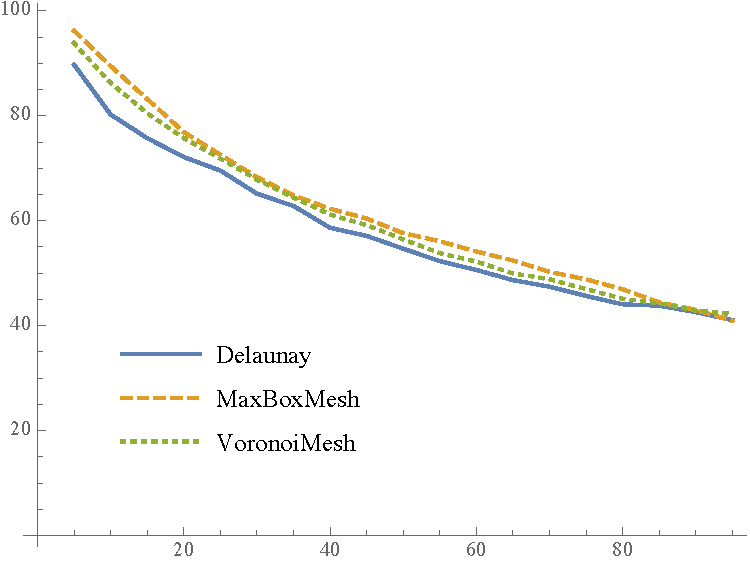
\includegraphics[width=0.4\textwidth,]{plot-KS-Failure-by-Training.pdf}};
%%     \node[below=of img, node distance=1cm, yshift=1cm] {Percentage of Training Data};
%%     \node[left=of img, node distance=0cm, rotate=90, anchor=center,yshift=-0.7cm] {\% Null Hypothesis Rejections};
%%   \end{tikzpicture}
%%   \caption{The performance of each algorithm on the KS test ($p=0.001$) with increasing amounts of training data averaged over all IOzone test types and ten random splits of the data. The training percentages range from 5\% to 95\% in increments of 5\%. Delaunay is the best performer until 95\% of data is used for training, at which Max Box mesh becomes the best performer by a fraction of a percent.
%%   \vspace{-.1cm}}
%%   \label{fig:ks_failure_by_training}
%% \end{figure}


%% \begin{figure}
%%   \begin{tikzpicture}
%%     \node (img)  {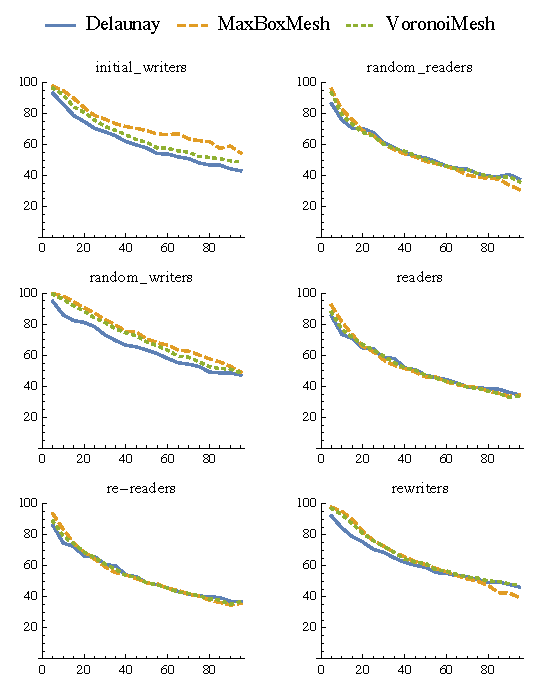
\includegraphics[width=0.4\textwidth,]{plot-KS-failure-by-training-and-test.pdf}};
%%     \node[below=of img, node distance=1cm, yshift=1cm] {Percentage of Training Data};
%%     \node[left=of img, node distance=0cm, rotate=90, anchor=center,yshift=-0.7cm] {\% Null Hypothesis Rejections};
%%   \end{tikzpicture}
%%   \caption{The percentage of null hypothesis rejections for predictions made by each algorithm on the KS test ($p=0.001$) over different IOzone test types with increasing amounts of training data. Each percentage of null hypothesis rejections is an average over ten random splits of the data. The training percentages range from 5\% to 95\% in increments of 5\%. The read test types tend to allow lower rejection rates than the write test types.
%%   \vspace{-.1cm}}
%%   \label{fig:ks_failure_by_training_and_test}
%% \end{figure}


\end{document}


